\documentclass[../../main.tex]{subfiles}
\begin{document}

\begin{flushright}
  \footnotesize\textit{【自動文字起こし・要確認】}
\end{flushright}

[解] $P(t, t^3)\ (t \in \mathbb{R})$ とおく．$P$ における接線 $l$ として
\[ l: y - t^3 = 3t^2(x - t) \]
である．$l$ 上の点 $(X,Y)$ が $L$ 上の点 $(x,y)$ にうつったとすると，
\begin{figure}[htb]
  \centering
  % t=0.4 の模式図．接線の傾きは 0.48，回転後の傾きは (0.48+1)/(1-0.48)．
  \begin{tikzpicture}[x=2.4cm, y=1.5cm, >=stealth, every node/.style={font=\small}]
    \coordinate (P) at (0.4,0.064);
    \draw[->, thick, gray!80!black] (-0.9,0) -- (1.4,0) node[right] {$x$};
    \draw[->, thick, gray!80!black] (0,-1.15) -- (0,1.5) node[above] {$y$};
    \draw[line width=1.4pt, blue!85!black, domain=-0.85:1.1, samples=90] plot (\x,{\x*\x*\x});
    \draw[teal!75!black, thick] (-0.2,-0.224) -- (1.12,0.4096) node[right] {$l$};
    \draw[orange!85!black, thick] (0.08,-0.847) -- (0.86,1.373) node[above] {$L$};
    \draw[orange!85!black, ->] ($(P)+(25.6:0.32)$) arc[start angle=25.6,end angle=70.6,radius=0.32];
    \node[above right=5pt, orange!85!black, font=\footnotesize] at (P) {$45^\circ$};
    \fill[blue!85!black] (P) circle (1.5pt);
    \node[below right=3pt] at (P) {$P$};
    \node[above left=2pt, blue!85!black] at (-0.58,-0.2) {$C:y=x^3$};
  \end{tikzpicture}
  \caption{$P$での接線$l$を反時計回りに$45^\circ$回転した直線$L$（図は$t=0.4$）}
\end{figure}
\begin{eqnarray*}
  \{ (X-t) + i(Y-t^3) \} &=& \dfrac{\sqrt{2}}{2}(1-i) \{ (x-t) + i(y-t^3) \} \\
  &=& \dfrac{\sqrt{2}}{2} \left[ \{ (x-t) + (y-t^3) \} + i \{ (y-t^3) - (x-t) \} \right] \\
  &=& \dfrac{\sqrt{2}}{2} \left[ (x+y-t-t^3) + i (-x+y+t-t^3) \right]
\end{eqnarray*}
から
\[ X-t = \dfrac{\sqrt{2}}{2}(x+y-t-t^3),\ Y-t^3 = \dfrac{\sqrt{2}}{2}(-x+y+t-t^3)\ (x, y, X, Y, t \in \mathbb{R}) \]
だから
\[ l: -x+y+t-t^3 = 3t^2 (x+y-t-t^3) \cdots \text{\textcircled{1}} \]
これが $y=x^3$ と $3$ 異交点を持つ時，\textcircled{1} に $y=x^3$ を代入した
\begin{eqnarray*}
  -x+x^3+t-t^3 &=& 3t^2 (x+x^3-t-t^3) \\
  (x-t) \{ 3t^2 (x^2+tx+t^2+1) - (x^2+tx+t^2-1) \} &=& 0 \cdots \text{\textcircled{2}}
\end{eqnarray*}
が $x$ について $3$ 実数解を持つ．したがって，$\{ \ \}$ 部を $f(x)$ として，$f(x)=0$ が $x \neq t$ に $2$ 異実解を持てば良い．
\[ f(x) = (3t^2-1)x^2 + (3t^3-t)x + (3t^4+2t^2+1) \]
だから，条件は，$f(x)=0$ の判別式 $D$ として
\[
  \begin{cases} f(t) \neq 0,\ 3t^2-1 \neq 0 \\ D > 0
\end{cases} \cdots * \]
である．
\[ f(t) = 9t^4+1 \neq 0 \ (\because t \in \mathbb{R}) \]
\begin{eqnarray*}
  D &=& t^2(3t^2-1)^2 - 4(3t^2-1)(3t^4+2t^2+1) \\
  &=& (3t^2-1) \left[ p(3p-1) - 4(3p^2+2p+1) \right] \ (p=t^2) \\
  &=& -(3p-1)(3p+2)^2
\end{eqnarray*}
だから $*$ に代入して，$3p+2>0$ とあわせて
\[ * \iff 3t^2 < 1 \iff -\dfrac{\sqrt{3}}{3} < t < \dfrac{\sqrt{3}}{3} \]
だから $P$ のハンイは下図太線部

\begin{figure}[htb]
  \centering
  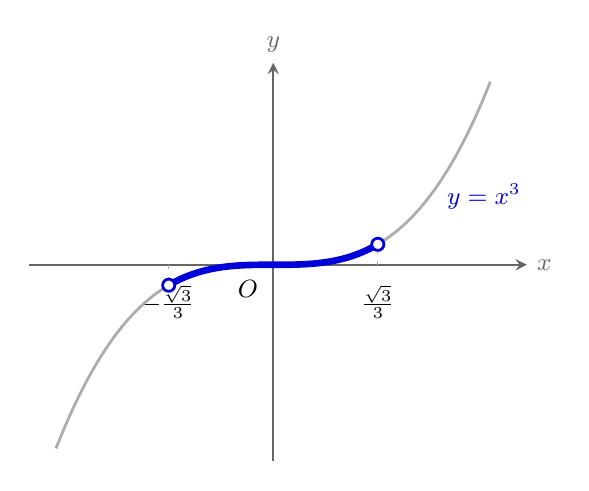
\begin{tikzpicture}[x=2.3cm, y=1.35cm, >=stealth, every node/.style={font=\small}]
    \draw[->, thick, gray!80!black] (-1.35,0) -- (1.4,0) node[right] {$x$};
    \draw[->, thick, gray!80!black] (0,-1.85) -- (0,1.9) node[above] {$y$};
    \draw[gray!65, line width=1pt, domain=-1.2:1.2, samples=100] plot (\x,{\x*\x*\x});
    \draw[blue!85!black, line width=2.4pt, domain=-0.57735:0.57735, samples=70]
    plot (\x,{\x*\x*\x});
    \draw[dashed, gray!65] (-0.57735,-0.19245) -- (-0.57735,0)
    (0.57735,0.19245) -- (0.57735,0);
    \filldraw[fill=white, draw=blue!85!black, line width=1pt]
    (-0.57735,-0.19245) circle (2.2pt) (0.57735,0.19245) circle (2.2pt);
    \node[below=4pt, font=\footnotesize] at (-0.57735,0) {$-\frac{\sqrt{3}}{3}$};
    \node[below=4pt, font=\footnotesize] at (0.57735,0) {$\frac{\sqrt{3}}{3}$};
    \node[right=3pt, blue!85!black] at (0.86,0.64) {$y=x^3$};
    \node[below left=2pt] at (0,0) {$O$};
  \end{tikzpicture}
  \caption{3つの異なる交点を与える$P$の範囲（青い部分，両端を除く）}
\end{figure}

\end{document}
